\section{Experiments}
\label{sec:experiments}

The objective of this experiment section is twofold:
\begin{itemize}[noitemsep, leftmargin=*]
\item To confirm the complexity of \LSEQ. Monotonic editing behavior should lead
  to a polylogarithmic growth of identifiers compared to the number of
  insertions. Time complexity should be logarithmic except for the lookup which
  is expected to be linear after monotonic editing.
\item To show the impact on the generated traffic on a real decentralized
  collaborative editor. We expect that both the identifier size and neighborhood
  size impact the traffic. Since the former grows polylogarithmically, and the
  latter grows logarithmically, we expect the traffic to scale in terms of
  the number of users and the number of operations.
\end{itemize}

We conducted the experiments using a JavaScript implementation directly usable
within web browsers. Part of the experiments ran on the \emph{Grid'5000} testbed
involving up till 601 instances of the editor distributed among 101 machines.


\subsection{Space complexity}

\begin{figure}
  \centering
  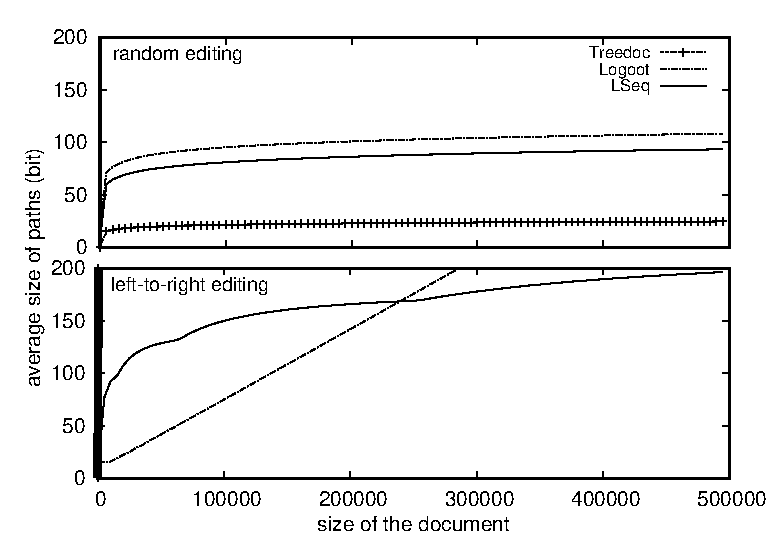
\includegraphics[width=0.8\textwidth]{./img/space.eps}
  \caption{\label{fig:space}Size of paths allocated by Treedoc, Logoot, and
    \LSEQ.}
\end{figure}



\begin{asparadesc}
\item [Objective:] To confirm the space complexity of \LSEQ's identifiers and to
  highlight the improvement over state-of-the-art.
\item [Description:] We consider two editing behaviors:
  \begin{inparaenum}[(i)]
  \item random which consists in inserting elements at random position in the sequence;
  \item left-to-right which consists in inserting elements at the end of the
    sequence.
  \end{inparaenum} We measure the average bit size of paths allocated by
  Treedoc~\cite{preguica2009commutative}, Logoot~\cite{weiss2009logoot}, and
  \LSEQ~\cite{nedelec2013lseq}. The generated documents reach half a million
  characters.
\item [Result:] Figure~\ref{fig:space} shows the results of the experiment. The
  x-axis denotes the size of the document. The y-axis denotes the average size
  of generated paths. The top figure shows the measurements of the random
  editing behavior while the bottom figure shows the measurements of the
  left-to-right editing behavior. As expected, we observe that random editing
  leads to logarithmic growth of paths whatever the allocation function. In
  addition, Treedoc allocates the smallest paths, followed by \LSEQ, followed by
  Logoot. Nonetheless, on left-to-right editing, paths allocated by Treedoc grow
  extremely quickly to such an extent that its plot merges with the
  y-axis. Logoot's paths grow slower but still linearly compared to the number
  of insertions in the document. We observe that \LSEQ exposes a better space
  complexity compared to the state-of-the-art, which eventually leads to smaller
  allocated paths.
\item [Reason:] The random editing leads to a balanced underlying structure,
  hence the logarithmic progression of paths allocated by the three
  strategies. In this case, Treedoc is better because it has an arity of $2^1$,
  for it is a binary tree. In this setup, \LSEQ starts with an arity of $2^8$
  while Logoot has an arity of $2^{16}$, hence \LSEQ allocating smaller paths than
  Logoot in random editing. The left-to-right editing behavior tends to
  unbalance the tree over insertions. In Treedoc, monotonic editing is the worst
  case scenario where each new path contains all paths allocated before
  it. Logoot is designed to handle left-to-right editing. It allocates paths but
  keeps space for upcoming insertions. Still, since its maximum arity is
  constant, the number of characters in a branch is constant, hence the linear
  growth of paths. On the opposite, \LSEQ doubles its arity at each level of the
  tree. The branch can store twice as much elements as its parent. Hence a
  growth that scales sublinearly compared to the number of insertions in the
  document.
\end{asparadesc}

\subsection{Time complexity}


\begin{asparadesc}
\item [Objective:] To confirm the time complexity of \LSEQ's operations. We
  expect good scalability of operations except for the lookup after monotonic
  editing.
\item [Description:] This experiment involves one user who performs operations
  on its local copy of the document. The benchmark ran on a MacBook Pro with 2.5
  GHz Intel Core i5, with Node.js 4.1.1 on Darwin 64-bit. For each operation, we
  create a document containing $I-1$ characters and measure the time taken by
  the $I^{th}$ operation. The operation set includes the lookup, the local part
  of an insertion, the remote part of an insertion, and the remote part of a
  deletion -- the local part of a deletion only consist of broadcasting the
  identifier. We perform the measurements multiple times on two kinds of
  documents. Firstly, a document generated by random editing, i.e. the
  underlying \LSEQ tree is balanced. Secondly, a document generated by monotonic
  editing, i.e. one branch per level of the \LSEQ tree is filled.  We focus on
  tendencies rather than absolute values. Javascript does a lot of on-the-fly
  optimization which we limit in order to show the real time contribution of
  each operation.
\item [Result:] Figure~\ref{fig:time} shows the result of this experiment. The
  x-axis denotes the number of insert operations performed before the measured
  operation. The y-axis denotes the average time taken by this operation. Both
  axis are on a logarithmic scale. The top part of the figure focuses on a
  structure filled with insertions following a random editing behavior while the
  bottom part of the figure focuses on a structure filled with insertions
  following a monotonic editing behavior. We observe that the measured values
  barely grow after random editing, regardless of the operation. On the other
  hand, while the local insertion after monotonic editing remains stable, we
  observe a linear growth with the lookup execution time, and a slower growth
  for both the remote insertions and the remote deletions.
\item [Reason:] After the insertions at random positions, the underlying tree of
  \LSEQ is balanced. Therefore, the range of influence of each operation is
  limited to a small subset of the elements composing the document. For
  instance, the lookup operation does not need to explore each element of the
  tree. Instead, it quickly discards a lot of irrelevant branches at each level
  of the tree because the index does not fall into their range. However, this
  remark does not hold when the insertions followed a monotonic editing
  behavior. Indeed, in this case, most elements are located in the one and
  deepest level of the tree. Thus, the lookup likely crawls to this level and
  then inspects each elements to count their children and actualize its current
  index. The remote operations measurements follow the same reasoning: they must
  perform a binary search at each depth of the tree; since the random editing
  structure is balanced, the average depth of the search is smaller compared to
  the structure resulting from monotonic editing behavior. Hence, a lower time
  complexity.
\end{asparadesc}

\begin{figure}
  \centering
  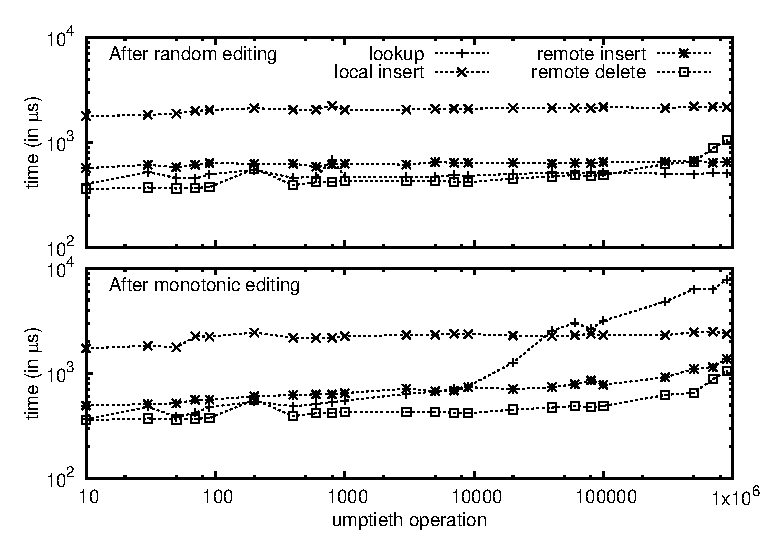
\includegraphics[width=0.8\textwidth]{./img/time.eps}
  \caption{\label{fig:time} Performance of the umptieth operation performed in
    \LSEQ.}
\end{figure}


% \ \\

% \begin{figure}
%   \centering
%   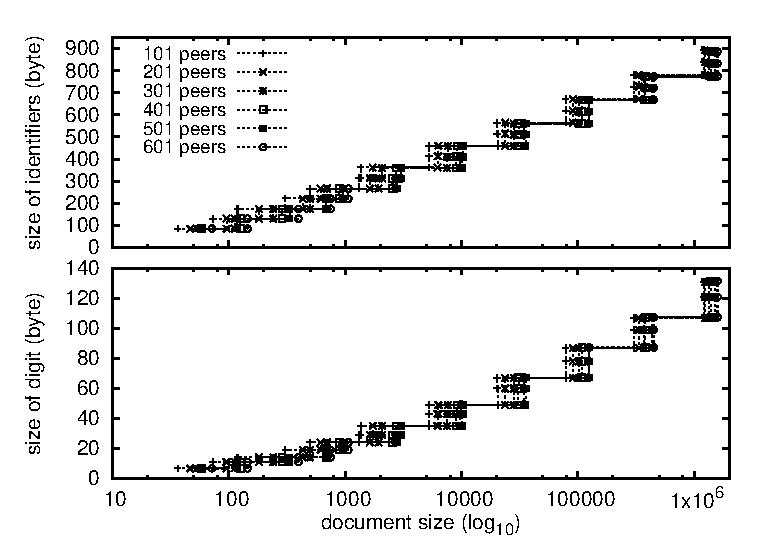
\includegraphics[width=0.8\textwidth]{./img/identifiers.eps}
%   \caption{\label{fig:identifiers} Size of \LSEQ's paths generated during
%     real-time editing sessions.}
% \end{figure}

% \begin{asparadesc}
% \item [Objective:] To confirm the space complexity of the identifiers generated
%   by \LSEQ. On the common monotonic editing behavior, we expect a
%   polylogarithmic growth compared to the document size.
% \item [Description:] The executions follow the previous experiment about the
%   neighborhood size. Thus, the experimentation comprises 6 runs with networks
%   including 101, 201, 301, 401, 501, 601 members. The editing session members
%   are repeatedly inserting new characters at the end of the document. The rate
%   of these operation is 100 operations per second distributed among
%   members. Thus, the experiment involving 101 members forces each member to
%   perform 1 insertion per second, while the experiment involving 601 members
%   forces each member to perform 1 insertion every 6 seconds. During the runs,
%   each author reports the byte-size of newly generated identifiers along with
%   the byte-size of its path in the exponential tree. \TODO{site, counter,
%     starting values of the exponential tree}.
% \item [Result:] Figure~\ref{fig:identifiers} shows the result of this
%   experimentation. The x-axis denotes the document size (which is equivalent to
%   the number of insert operations since the members do not perform removals) on
%   a decimal logarithmic scale. Thus, the document grows from empty to above a
%   million characters. The y-axis of the top part of the figure denotes the
%   byte-size of the identifiers while the bottom part of the figure denotes the
%   byte-size of the path only. First, we observe that all plots are very close
%   from each other. Hence, the size of identifiers does not depend of the number
%   of participants. Second, we observe that the identifiers grows
%   polylogarithmically compared to the size of the document. Indeed, the bottom
%   part of Figure~\ref{fig:identifiers} shows that the increment step of the
%   generated paths is slowly increasing during the experiment. It empirically
%   exposes a small surlinear behavior when the x-axis is on a logarithmic
%   scale. Hence the polylogarithmic curve. Finally, we can observe that \LSEQ
%   generates paths the size of which is small comparatively to the whole
%   identifier that includes site identifiers and counters to guarantee
%   uniqueness.
% \item [Reason:] The curves of the byte-size are close because the identifiers
%   of \LSEQ do not depend of whom created it nor the number of authors involved
%   in the document editing. They only depend of the position of insertions which
%   globally corresponds to the editing behavior. In this case, the highlighted
%   editing behavior is a monotonic left-to-right editing, i.e., repeated
%   insertions at the end of the document. This kind of behavior tends to
%   unbalance the tree by filling only one branch per level of the
%   tree. Fortunately, since the tree exponentially grows (each element has twice
%   as much children as its parent), the path growth slowly decreases over
%   insertions. Nevertheless, it costs one additional bit to encode each
%   concatenation of the path, hence the path growth on the bottom part of the
%   figure. The identifiers are much heavier than the path they carry because they
%   also includes a list of pairs to guarantee the uniqueness of identifiers and a
%   global total order. Each member generates its own globally unique identifier
%   (with high probability) without relying on any remote service. As such, they
%   require large identifiers that does not collide with remote members.
% \end{asparadesc}

\subsection{Communication complexity}

\begin{figure}
  \centering
  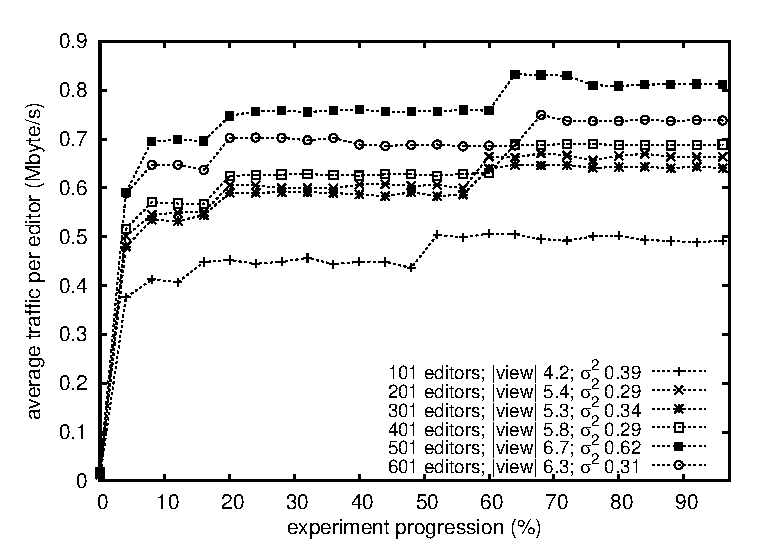
\includegraphics[width=0.8\textwidth]{./img/communication.eps}
  \caption{\label{fig:traffic} Average traffic per second at each editor during
    real-time editing session.}
\end{figure}

\begin{asparadesc}
\item [Objective:] To show that \LSEQ, along with other components, allows
  building a decentralized collaborative editor that scales well in terms of
  number of participants and document size. We expect the traffic to grow
  polylogarithmically compared to the document size, multiplied by a logarithm
  compared to the number of participants. The former being the contribution of
  \LSEQ and the latter being the contribution of messages propagation.
\item [Description:] This experimentation concerns networks from 101 members to
  601 members. Each editing session collaboratively writes a document of over a
  million of characters by repeatedly inserting new characters at the end of the
  document. We measure the average outgoing traffic of members. 100 operations
  are performed per second uniformly distributed among participants. The
  editing sessions last 7 hours. The documents reach millions of characters.
\item [Result:] Figure~\ref{fig:traffic} shows the result of this experiment.
  The x-axis denotes the experiment progression. The y-axis shows the average
  outgoing traffic generated by members. As expected, we observe two results:
  \begin{inparaenum}[(i)]
  \item the growth of each individual plot corresponds to a polylogarithmic
    increasing due to the paths allocated by \LSEQ;
  \item the growth between plot corresponds to a logarithmic increasing due to
    the neigbhorhood maintained by each editor using \SPRAY.
  \end{inparaenum}
  Hence, \CRATE scales in terms of number of participants and number of
  operations.
\item [Reason:] When an outsider joins the network, it injects a number of
  connections roughly logarithmic compared to the current network size. When it
  generates an operation, it sends its result to its neighborhood. Since the
  identifiers grow polylogarithmically compared to the document size, and since
  the neighborhood grows logarithmically compared to the network size, it
  multiplies the polylogarithm with the logarithm. When a member receives such
  operation, and it receives it for the first time, it sends it to its
  neighborhood. Therefore, for each operation performed by any member, the rest
  of the members will send the result of the operation to all their respective
  neighborhood once. The network load is balanced among users. Furthermore, it
  scales in number of editing session members and document size.
\end{asparadesc}

%%% Local Variables:
%%% mode: latex
%%% TeX-master: "../paper"
%%% End:
